\documentclass{article}
\usepackage{titlesec}
\usepackage{titling}
\usepackage{graphicx}
\usepackage{hyperref}

\titleformat{\section}
{\huge\bfseries}
{}	%{\thesection}
{0ex}
{}[\titlerule]

\titleformat{\subsection}
{\bfseries\Large}
{$\bullet$}
{0ex}
{}

\titleformat{\subsubsection}[runin]
{\bfseries}
{}
{0ex}
{}[:]

\renewcommand{\maketitle}{
\begin{center}
{\huge\bfseries\theauthor}
\vspace{.25em}

\texttt{sayanthecomputerguy@gmail.com}\\
\textit{+91 8583817369}\\
\url{https://thescienceuniverse.com/}
\end{center}
}


\begin{document}

\title{R\'esum\'e}
\author{Sayan Shankhari}
\maketitle

\begin{figure}[h]
\begin{center}
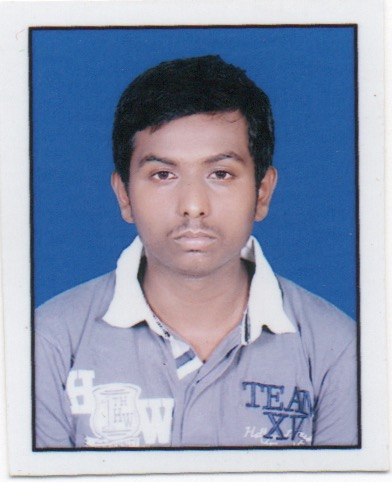
\includegraphics[width=3.5cm]{Sayan.jpeg}
\caption{sayan.jpeg}
\end{center}
\end{figure}

\section{Area of Interest}
Artificial Intelligence\\
Webpage Designing\\
Internet of Things\\
Cryptography\\
Networks\\
Computer Architecture\\
Mini/Micro Hardwares, Microcontrollers \& Embedded Systems

\section{Technical Skills}

\subsection{Work Flow}
Terminal, Vim, Git

\subsection{Languages}
\subsubsection{Programming}
C, C++, Java, VHDL, Arduino, MatLab(all at Intermediate Level)
\subsubsection{Markup}
{\LaTeX}, HTML, CSS, JavaScript, PHP (All at Beginner Level)
\subsubsection{Scripting}
Python, Shell(All at Beginner level)

\subsection{Other}
JDBC, Oracle SQL, MySQL(all at Intermediate Level)

\subsection{Multimedia}
\subsubsection{Image}
\subsubsection{Audio}
Very basic use of FFmpeg, iMovie for audio processing
\subsubsection{Video}
Very basic use of FFmpeg, iMovie for video processing\\For YouTube audio-books

\section{Projects}
\subsection{Computer Vision (2018-present)}
\subsubsection{Objective} Analysis Videos of Real Games
\subsubsection{Status} Ongoing
\subsubsection{Guide} Dr. Oishila Bandyopadhyay
\subsubsection{Language/Sofware used} Python, OpenCV

\subsection{RobBot (2018-present)}
\subsubsection{Objective} Making an Arduino-based Robot Software \& Hardware
\subsubsection{Status} Ongoing
\subsubsection{Guide} Dr. Oishila Bandyopadhyay
\subsubsection{Language/Sofware used} Java, C, JDBC, MySQL, Arduino

\subsection{Fault Analysis on mCrypton \& SEA}
\subsubsection{Objective} Implementing and Analysis on Fault Attack on mCrypton \& SEA
\subsubsection{Status} Implemented, not Analyzed
\subsubsection{Guide} Dr. Sandip Karmakar
\subsubsection{Language/Sofware used} C

\subsection{Software design \& Analysis of Micro Rain Rader (2016-'17)}
\subsubsection{Status}	Terminated
\subsubsection{Language/Sofware used} Java, C

\subsection{Scientific Calculator (2016-'17)}
\subsubsection{Status}  Done
\subsubsection{Language/Sofware used} Java

\section{Education}
\subsection{Bachelor of Technology (2015-present)}
\subsubsection{Gov.}	M.H.R.D.
\subsubsection{Collage}	Indian Institute of Information Technology Kalyani
\subsubsection{Semester I(SGPA)}	7.97
\subsubsection{Semester II(SGPA)}	9.46
\subsubsection{Semester III(SGPA)}	%NULL
\subsubsection{Semester IV(SGPA)}	8.14
\subsubsection{Semester V(SGPA)}	8.42
%\subsubsection{Semester VI(SGPA)}	%NULL
%\subsubsection{Semester VII(SGPA)}	%NULL
%\subsubsection{Semester VIII(SGPA)}	%NULL

\subsection{Higher Secondary Examination (2013-'15)}
\subsubsection{Gov.}	W.B.C.H.S.E.
\subsubsection{School}	Ranghat Anchal High School
\subsubsection{Final Marks(\%)}	87.8

\subsection{Secondary Examination (2007-'15)}
\subsubsection{Gov.}	W.B.B.S.E.
\subsubsection{School}	Ranghat Anchal High School
\subsubsection{Final Marks(\%)}	90.2

\section{Work Experience}
N/A

\section{Achievements}
- Qualified JEE Advanced 2015\\
- Participator \& Volunteer in School level Games

\section{Interests \& Hobbies}
\subsection{Reading}
Science Articles in Internet\\
Ancient Inventions\\
Detective \& Adventurous\\
Ancient History
\subsection{Solving}
Riddles \& Puzzles in Articles \& Videos
\subsection{Games}
\subsubsection{Physical} Cricket
\subsubsection{Logical} Tic-Tac-Toe, Chess, Shudoku, Cards
\subsection{Designing} Own Website

\section{Personal Details}
Full Name: Sayan Shankhari\\
Father: Ashim Shankhari\\
Mother: Sabita Shankhari\\
DOB: 18/09/1997\\
Residential Address: Baikola, N 24 Parganas, W.B., 743270\\
Current Address: B-14/469 (Magnet House), Kalyani, W.B., 741235\\
India\\

\section{Profiles}
\subsection{Programming}
\subsubsection{GitHub}
\url{https://github.com/Sayan0Programmer/}
\subsubsection{GeeksForGeeks}
\url{https://auth.geeksforgeeks.org/user/SayanShankhari/}
\subsubsection{InterviewBit}
\url{https://www.interviewbit.com/profile/Sayan0Programmer}
\subsubsection{Codechef}
\url{https://www.codechef.com/users/the01coder/}
\textit{Newly created}
\subsubsection{HackerRank}
\url{https://www.hackerrank.com/Sayan0Programmer/}
\textit{Newly created}
\subsection{Social}
\subsubsection{Twitter}
\url{https://twitter.com/twitting\_s}
\subsubsection{Linkedin}
\url{https://www.linkedin.com/in/sayan0programmer/}

\section{References}
\subsection{Dr. Sandip Karmakar}
Assistant Professor(Dept. of CSE \& IT), IIIT Kalyani\\
Kalyani, 741235, W.B., India\\
Email: \texttt{sandip1kk@gmail.com}
\subsection{Dr. Hafizul Islam}
Assistant Professor(Dept. of CSE \& IT), IIIT Kalyani\\
Kalyani, 741235, W.B., India\\
Email: \texttt{hafi786@iiitkalyani.ac.in}
\subsection{Dr. Imon Mukherjee}
Assistant Professor(Dept. of CSE \& IT), IIIT Kalyani\\
Kalyani, 741235, W.B., India\\
Email: \texttt{imon@iiitkalyani.ac.in}

\end{document}
